\documentclass[11pt,a4paper]{article}

\usepackage[margin=2.4cm]{geometry}
\usepackage[T1]{fontenc}
\usepackage[utf8]{inputenc}
\usepackage{lmodern}
\usepackage{amsmath, amssymb}
\usepackage{booktabs}
\usepackage{graphicx}
\usepackage{float}
\usepackage{xcolor}
\usepackage[hidelinks]{hyperref}
\usepackage{microtype}

\setlength{\emergencystretch}{3em}
\graphicspath{{figures/}}

\definecolor{verdict}{HTML}{C1666B}

\title{SafetyDial Phase 0 Report\\[0.4em]
  \large Does the Safety-Gymnasium locomotion suite support the proposal's premise?}
\author{Sachin Mohan \\ Student No. 2699183 \\
  Supervised by Geraud Nangue Tasse \\ University of the Witwatersrand}
\date{20 September 2026}

\begin{document}
\maketitle

\begin{abstract}
Phase 0 was built to test, cheaply and early, whether the environment chosen in the revised
proposal can support its central claim. The answer is robot-dependent, and the proposal picked the
wrong robot. Walker2d, the environment the revised proposal builds its argument around, has no
irreversible failures at all: given a four second horizon and a competent planner it recovers from
lying on the ground in every case tested, and recoverability does not fall below 0.88 at any point
either side of the benchmark's failure flag. Hopper does have a genuine irreversibility boundary,
but it sits roughly 40 steps \emph{after} the flag fires, and about half of well-fallen Hopper
states are irrecoverable. So the premise survives, on a different robot, with the failure set
displaced from where the benchmark says it is. This report records what was built, what was
measured, the corrections that measurement forced, and what follows.
\end{abstract}

\section{Verdict}

The revised proposal rests on a contrast: that the velocity cost is \emph{extrinsic and
recoverable} while falling is \emph{intrinsic and irreversible}, and that this split, inside a
single recognised benchmark, gives a labelled mode and an unlabelled mode for the transfer
experiment.

The second half of that contrast is false for Walker2d, which is the robot the proposal names.
Measured on settled-fallen states, with the robot's torso on the floor:

\begin{table}[H]
\centering
\begin{tabular}{lcc}
\toprule
Robot & irrecoverable at $H=250$ (2\,s) & at $H=500$ (4\,s) \\
\midrule
Walker2d & \textbf{0.000} & \textbf{0.000} \\
Hopper   & 0.333 & 0.167 \\
\bottomrule
\end{tabular}
\caption{Fraction of fallen states from which no action sequence was found. 30 states per cell,
full CEM search on the true simulator. Walker2d is at zero for both horizons.}
\end{table}

Hopper is the exception, and it is the useful one. Sweeping either side of the failure flag with
40 states per point (Figure~\ref{fig:offset}), Walker2d never drops below $0.88$ recoverable
anywhere, while Hopper falls from $1.000$ at the flag to $0.450$ at $+40$ steps. Hopper therefore
has a real irreversibility boundary; it simply is not where \texttt{terminated} says it is.

\paragraph{What follows.} Walker2d cannot support the proposal's experiment and should be dropped.
Hopper can, with the failure set taken from the oracle rather than from the termination flag. This
is the outcome Phase 0 exists to detect, and detecting it cost one day rather than surfacing in
Stage 2 in November.

\section{What was built}

2{,}964 lines across seven helper modules and five scripts, all lint-clean, with no \texttt{src/}
package (per the project's own rule that new code lives in \texttt{experiments/helpers/}).

\begin{table}[H]
\centering
\small
\begin{tabular}{ll}
\toprule
Module & Role \\
\midrule
\texttt{locoEnv.py} & Vendored Safety-Gymnasium velocity task; thresholds; stack fingerprint \\
\texttt{locoCollect.py} & State-only HDF5 writer and rollout loop \\
\texttt{locoPolicies.py} & Uniform \texttt{act(obs)} adapters \\
\texttt{locoData.py} & Lazy-render dataset; worker-safe EGL; render fingerprint \\
\texttt{locoMetrics.py} & Gate 0 statistics, disjointness lift, matched pairs, AUROC \\
\texttt{oracle.py} & The recoverability oracle. Five search tiers. Evaluation only \\
\texttt{equivCheck.py} & Vendored-env equivalence gates; numpy-only, loads under both stacks \\
\bottomrule
\end{tabular}
\end{table}

\subsection{Storage: state, not pixels}

Restoring \texttt{(qpos, qvel)} and replaying the recorded actions reproduces \texttt{qpos} to
$7.4\times10^{-15}$, and renders from a restored state are bit-identical, so pixels need never be
written to disk. Walker2d has \texttt{na == 0}, making \texttt{(qpos, qvel)} the complete state.

\begin{figure}[H]
\centering
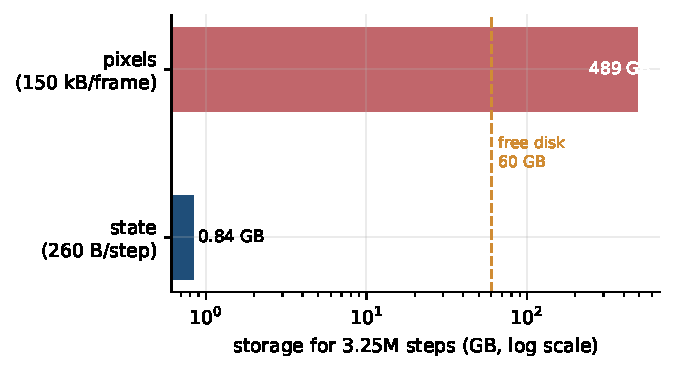
\includegraphics[width=0.62\textwidth]{fig_storage.pdf}
\caption{Storing state costs 260 bytes per step against 150\,kB for a $224\times224$ frame. The
pixel route does not fit in the available disk; the state route is free. Frames regenerate at
3{,}101 per second, and the dataset delivers 607 samples/s single-process, four to seven times
what the GPU consumes.}
\end{figure}

\subsection{The vendored environment}

\texttt{safety-gymnasium==1.0.0} cannot be installed alongside \texttt{stable-worldmodel}: it
carries hard \texttt{==} pins on \texttt{gymnasium 0.28} and \texttt{mujoco 2.3}, so
\texttt{uv lock} fails outright. The velocity task is therefore copied verbatim rather than
depended on. \texttt{walker2d.xml} has md5 \texttt{7fb5491cd0097896df56653c3d0f18a0} on both
stacks, with identical model scalars, and an equivalence harness gates cost sums, termination
indices, observations, velocities and rewards.

\section{The recoverability oracle}

The environment's own \texttt{terminated} flag cannot serve as ground truth for irreversibility.
It is a threshold on torso height and pitch, and both decode from a raw $32\times32$ grayscale
frame at $R^2 = 0.99$, so scoring a detector against it is close to circular.

Recoverability is therefore measured directly. From a saved MuJoCo state, with termination
disabled, the oracle searches for an action sequence that returns the robot to a settled upright
pose. Any success proves recoverability, so the search is one-sided: more search can only shrink
the irrecoverable set, never grow it.

\paragraph{Recovery predicate (Walker2d).} $1.00 \leq z \leq 1.80$, $|\text{pitch}| \leq 0.50$,
$\max|\dot q_{0:3}| \leq 5.0$, held for 25 consecutive steps. Every constant sits strictly inside
the environment's own health set ($0.8 < z < 2.0$, $|\text{pitch}| < 1.0$), which is what stops
the oracle from restating \texttt{terminated}.

\paragraph{Five tiers, short-circuiting on first success.}
\textbf{T0} replays the actions that actually followed the state, a certificate rather than a
search; \textbf{T$\pi$} a trained controller; \textbf{T1} constant torques; \textbf{T2} low-pass
random torques; \textbf{T3} CEM over ten control knots interpolated to the horizon, on the true
simulator. The knot parameterisation is essential: the raw space is 1500-dimensional at $H=250$
and CEM does not work there, while ten knots makes it 60-dimensional.

Validation V1 (benign upright states must come back recoverable) reaches $1.000$ on 40 states,
against $0.92$ for the original design. The T0 certificate makes it 59 times cheaper, 4\,ms per
state against 235\,ms.

\section{Findings}

\subsection{The benchmark declares failure long before the robot falls}

\begin{figure}[H]
\centering
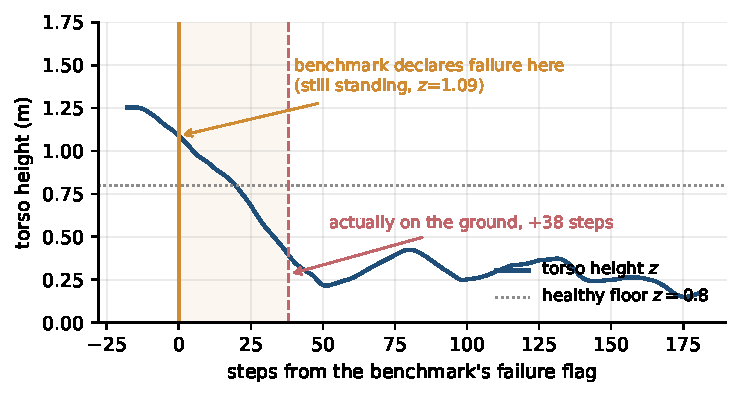
\includegraphics[width=0.8\textwidth]{fig_timeline.pdf}
\caption{One episode, collected with termination disabled so it continues past the benchmark's
cutoff. The flag fires while the torso is still at $z \approx 1.09$, leaning past 55 degrees. The
robot does not reach the ground for roughly another 38 steps.}
\end{figure}

\subsection{Falling is not irreversible}

\begin{figure}[H]
\centering
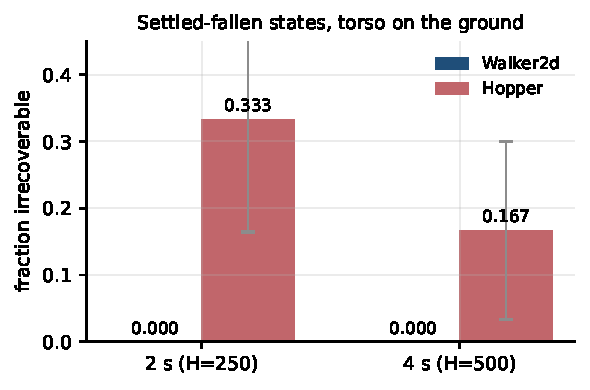
\includegraphics[width=0.62\textwidth]{fig_horizon.pdf}
\caption{Irrecoverable fraction on settled-fallen states, by robot and search horizon. Error bars
are normal approximations at $n = 30$. Walker2d is at zero for both horizons; Hopper declines
from 0.333 to 0.167 as the horizon doubles, so what is being measured is the time recovery takes,
not whether it is possible.}
\end{figure}

\begin{figure}[H]
\centering
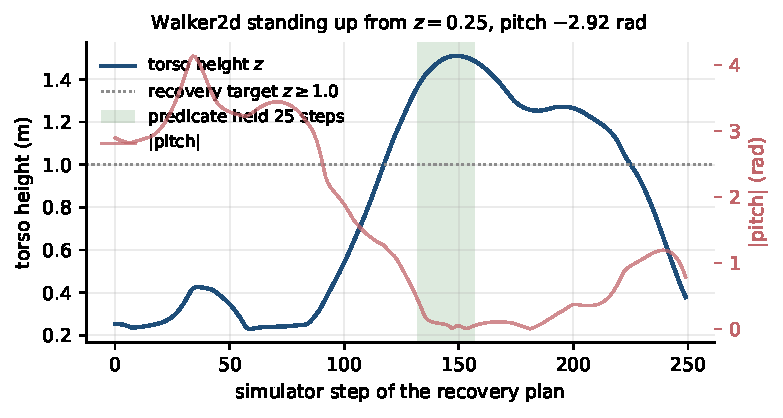
\includegraphics[width=0.8\textwidth]{fig_recovery.pdf}
\caption{A replayed recovery. The robot starts lying on the ground, upside down, and every action
in the plan is inside $[-1, 1]$, the same range any policy has. It rolls, pushes off and stands.
This is real physics rather than a simulator exploit: MuJoCo's Walker2d is a planar model with
gear-100 actuators and no self-collision, so it can right itself.}
\end{figure}

\subsection{Recoverability either side of the failure flag}

\begin{figure}[H]
\centering
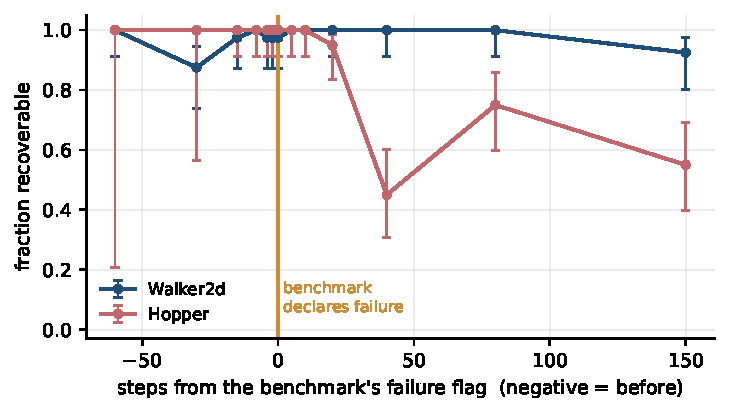
\includegraphics[width=0.85\textwidth]{fig_offset.pdf}
\caption{Fraction of states from which a recovery was found, against offset from the benchmark's
failure flag. Error bars are Wilson 95\% intervals at $n=40$ per point. If the flag marked a
transition into irreversibility, these curves would fall sharply at zero. Walker2d never moves:
recoverability stays near one on both sides, including 150 steps after the flag with the robot on
the ground. Hopper does fall, but late, from $1.000$ at the flag to $0.450$ at $+40$ steps, so its
irreversibility boundary is real and is displaced roughly 40 steps past where the benchmark places
it. The Hopper curve is not monotone beyond $+40$; at $n=40$ those points are within each other's
intervals and the sampled configurations differ.}
\label{fig:offset}
\end{figure}

\subsection{Mode A and Mode B are not disjoint}

\begin{figure}[H]
\centering
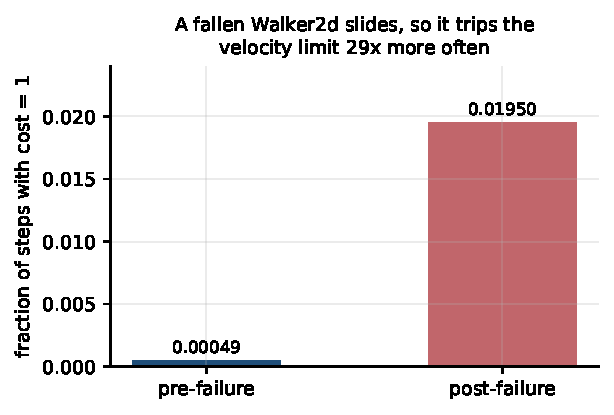
\includegraphics[width=0.62\textwidth]{fig_cost.pdf}
\caption{Cost rate before and after the failure. This asymmetry is what inverted the Gate 0
statistic: control windows were being drawn from the post-failure region, so the denominator was
measuring cost caused \emph{by} the fall.}
\end{figure}

\textbf{This corrects a number reported earlier in the work.} An initial run gave a disjointness
lift of $0.288$, that is, cost appearing \emph{anti-correlated} with imminent failure, which would
have been ideal for the transfer experiment. It was a bug. Corrected, with control windows
confined to the pre-failure phase and length-matched to the numerator:

\begin{table}[H]
\centering
\begin{tabular}{lc}
\toprule
Quantity & Value \\
\midrule
cost rate, pre-failure phase & $0.00049$ \\
$P(\text{cost in the 125 steps before failure})$ & $0.035$ \quad (7 of 200 episodes) \\
$P(\text{cost in a matched control window})$ & $0.000$ to $0.001$ \\
disjointness lift & 35 to $\infty$ across control seeds \\
\bottomrule
\end{tabular}
\caption{Gate 0 required lift $\leq 2.0$. Both rates are very small, so the ratio is unstable and
the honest statement is that the gate fails, not that the lift takes any particular value.}
\end{table}

Read carefully: cost is \emph{rare} before a failure in absolute terms, but when it does occur it
is concentrated immediately before one. Note also that this is measured under a crude
scripted-forward policy that drives maximum torque, accelerates past the limit and then trips; a
velocity-constrained policy would plausibly behave differently.

\section{Corrections forced by measurement}

\begin{enumerate}
  \item \textbf{The velocity cap applies to the root degrees of freedom only.} Walker2d joint
    velocities routinely exceed 10\,rad/s in normal gait, so an all-DOF cap turned ``recovered''
    into ``recovered and then stood perfectly still''. Measured: 91\% of benign states satisfy an
    all-DOF cap against 98.9\% for a root-only cap, and that 91\% was exactly the 92\% figure an
    earlier pilot had reported as its validation ceiling.
  \item \textbf{A certificate tier was added.} Pure search systematically under-detects
    recoverability for \emph{dynamic} states, because a robot in mid-gait needs an actual
    balancing controller to stay upright and zero torque simply drops it.
  \item \textbf{Collection runs with termination disabled.} The rollout records state
    \emph{before} each action, so \texttt{terminated[t]} means ``action $t$ made it unhealthy''
    while \texttt{qpos[t]} is the last \emph{healthy} state, and the episode then ends. Every row
    in such a dataset is healthy: it contains no failures at all. This produced a false alarm in
    which states at \texttt{terminated == 1} came back 96\% recoverable and read as the premise
    collapsing; they were healthy standing robots.
\end{enumerate}

\section{Adversarial audit}

A five-dimension audit with three independent skeptics per finding: 134 agents, 43 findings
raised, and roughly two thirds refuted under verification. Defects confirmed and fixed:

\begin{table}[H]
\centering
\small
\begin{tabular}{p{1.6cm}p{12.4cm}}
\toprule
Severity & Defect \\
\midrule
critical & \texttt{disjointness\_lift} drew control windows from the post-failure region,
  inverting Gate 0 from fail to pass \\
high & The recovery predicate had \emph{no upper $z$ bound}, so a ballistic arc could satisfy it:
  25 steps is only 0.2\,s of flight \\
high & Oracle labels were not reproducible. \texttt{set\_state} leaves \texttt{qacc\_warmstart}
  dirty, so the same rollout returned $-1.4618128503645678$ or $\ldots664$ depending on what ran
  before \\
high & The G4 equivalence gate was inverted: \texttt{first\_term} is $-1$ when no termination
  occurs, so ``reference terminated at step 0, test never terminated'' computed as an off-by-one
  and was excused as floating-point noise \\
high & The equivalence harness emitted observations, velocities, rewards and per-step costs,
  shipped them across, then compared only totals \\
high & T2's low-pass filter had no gain compensation: at $\beta = 0.9$ it commanded rms torque
  $0.132$ out of $1.0$, making the search four times weaker than intended \\
medium & Truncated rollouts returned \texttt{margins.max()}, an optimistic and different quantity
  from the windowed minimum they claimed to be \\
medium & CEM rollouts were excluded from the rollout count, so the budget-saturation check read a
  near-constant \\
\bottomrule
\end{tabular}
\end{table}

Two items are recorded rather than fixed: the lead-time statistic is a minimum over a sparse
offset grid and is censored, so it understates; and the hopeless early exit is the one place the
oracle's one-sidedness is an assumption rather than a guarantee.

\section{Where this leaves the project}

The oracle and the pipeline are sound and environment-agnostic. The environment is not. Four
options:

\begin{enumerate}
  \item \textbf{Controller-relative viability.} Keep Safety-Gymnasium and define irrecoverable as
    ``outside the viability kernel of a realistic controller class'' rather than ``no omniscient
    planner can recover''. Viability kernels in control theory are always defined relative to
    admissible controls, and a safety filter protects a \emph{specific} policy, so this is
    arguably the right object. The T$\pi$ tier already implements it. The cost is that the failure
    set stops being purely a property of the dynamics.
  \item \textbf{OGBench-Cube.} The August proposal's environment. A cube pushed off the table is
    genuinely irrecoverable. The cost is the loss of published safe-RL baselines.
  \item \textbf{Report the negative result.} ``Standard safe-RL locomotion benchmarks have no
    irreversible failures, and their termination flags are hand-set constants a competent
    controller recovers from.'' Surprising, checkable, and largely already done. The cost is that
    it becomes a benchmark critique rather than the Safety Dial thesis.
  \item \textbf{Add genuine irreversibility to the environment.} The cost is that it is no longer
    the literal published benchmark, which undercuts the reason for choosing it.
\end{enumerate}

On the evidence here, option 1 applied to \textbf{Hopper} is the shortest path: the environment,
the baselines and the whole pipeline survive, and the only change is that the failure set comes
from the oracle rather than from \texttt{terminated}. That change is not a workaround, it is the
proposal's own thesis, and Figure~\ref{fig:offset} is the evidence that the two sets genuinely
differ. Walker2d should be dropped rather than defended.

\section*{Reproducing}

{\small
\begin{verbatim}
# storage and replay invariants
uv run python experiments/scripts/verify_replay.py
# the full Phase 0 triage
uv run python experiments/scripts/run_triage.py
# every figure in this report
uv run python experiments/scripts/make_phase0_figures.py
\end{verbatim}
}

The numbers behind every figure are committed beside it in \texttt{docs/phase0/data/}, so a plot
can be re-made or checked without re-running the simulation that produced it. Supporting records:
\texttt{notes/phase0Report.md} (the same material in prose),
\texttt{notes/safetyGymLocomotion.md} (measured environment facts) and
\texttt{notes/terminationIsNotIrreversibility.md} (the finding in detail).

\end{document}
